\Chapter{Koncepció}

A dolgozat témájának megértéséhez elsősorban érdemes betekintést nyerni az eredeti, nem-inverz problémába is. Az obejktumfelismerésről csupán egy kis áttekintés olvasható az alábiakban, majd az irodalomkutatásom során fellelt munkák alapján bemutatásra kerülnek az inverz problémában elért eredmények. Az eredmények bemutatása betekintést nyújt a téma lehetőségeibe és kutatási irányaiba.

\Section{Az objektumfelismerés}
Az objektumfelismerés célja a számítógépes látás esetében, hogy egy gépi tanulásos modell egy vizsgált képen meghatározza a képen található objektumokat. Egyszerűbb esetben osztályozási feladatról beszélhetünk, amely során a bemeneti képeket egy-egy diszkrét címkével látja el a modell. A modell kimeneteként rendszerint az osztályokhoz tartozó valószínűségi értékeket kaphatjuk meg. Amennyiben a képen található objektum környezetéről feltételezzük, hogy nem hordoz számunka lényeges információkat, úgy a címkék használata elegendő lehet bizonyos feladatoknál. Viszont előfordulhat olyan alkalmazási környezet is, amikor a bemeneti képeken nem csupán egyetlen objektum található és minden fellelhető objektumhoz szeretnénk címkét rendelni. Ilyen esetekben a felismert objektumokat különféle annotációkkal láthatja el a modell. Legtöbbször a megtalált objektumok pozícióiról is adhat kimenetet, az azonosított elemeket befoglaló dobozokkal \cite{redmon2016you} vagy pixel-szinten is jelölheti a modell, az utóbbi esetben szemantikus szegmentációról beszélhetünk \cite{long2015fully}.

A képek osztályozásához általánosságban \textit{konvolúciós} hálózatot szokás alkalamzni. A konvolúciós rétegeket tartalmazó modell ezen rétegek segítségével nyeri ki az osztályozási művelet elvégzéséhez szükséges képi-jellegzetességeket. A digitális képek $n \times m$-es mátrixokként vannak reprezentálva, a mátrix egyes pontjai pedig szürkeárnyalatos képek esetében a pixel intenzitásának értékei, színes képek esetén pedig az adott színkeverés alapján a színcsatornák értékei. A konvolúciós rétegek a kernelek és a filterek segítségével oly módon nyerik ki a bemeneti képek jellegzetességeit, hogy figyelembe veszik a pixelek szomszédságait, ezáltal a képeken található információt egy kisebb dimenziószámú leírásba transzformálja. A kisebb dimenzióban reprezentált adatokon az osztályozási feladat egyúttal könyebben elvégezhető, másfelől a megfelelően összeállított jellegvektorok segítségével a képen található információ általánosabb formáját kapja meg az osztályozó, csökkentve annak a veszélyét, hogy a modell jellegtelen pixelekre tanulja be az egyes osztályoka.

% Konvolúció ábra?
% Vagy ide jöhetnének szemléltetésképpen ábrák a munkákból?

Kiemelném az \textit{Inception modell}-t \cite{szegedy2015going}, amely a Google kutatói által kifejlesztett mély konvolúciós hálózat. Fő céljuk egy olyan modell megalkotása volt, amely az \textit{ImageNet} adathalmaz \cite{deng2009imagenet} 1000 darab osztályára megoldja az osztályozási feladatot. Az eredeti modell 2014-es megjelenése óta három további verziót is megélt (v2/v3 \cite{szegedy2016rethinking}, v4 \cite{szegedy2017inception}). A modell az inverz probléma egyes megoldásai során is szerepet kap, így a dolgozat során a későbbiekben is említésre kerül.

Az irodalomkutatás során fellelt eredmények küzöl a legfigyelemreméltóbb eredmény a CLIP \textit{zero-shot} osztályozó \cite{radford2021learning}, amelyet az internetről összegyűjtött képeken és a hozzájuk tartozó szöveges leírásokon tanítottak be. A CLIP modell képes rövid leírásokat adni a kép tartalmáról és az egyes mondatokat valószínűségi értékekkel látja el. Vagyis a különféle annotációk helyett természetes-nyelvi leírásokat ad kimenetként egy-egy képhez. A modell az inverz problémakör egyes megvalósításában is feltűnik majd, amelyeket a következő alfejezetben ismertetek.

\Section{Az objektumfelismerés inverz problémája}

Az objektumfelismerés inverz problémája alatt azt a feladatot értjük, amely során csupán a képekre vonatkozó információk állnak redelkezésünkre és ezen adatok alapján a gépi tanulásos modellnek a lehető legjobban kell reprezentációt kell nyújtania egy-egy kimeneti kép formájában.
Ehhez nem csupán a bemeneti, általában természetesnyelvi szöveget kell értelmeznie a modellnek, hanem a képek kigenerálásának módja is egy megoldandó feladat.
A jelenlegi eredmények alapján különféle megközelítéseket láthatunk a problémára. Az eredményeket többféle szempont szerint is csoportosíthatjuk. Mivel a megoldandó probléma alapvetően is két részre osztható: a bemeneti adatok feldolgozása és a kimeneti kép generálása, így a a csoportosításokat ezek alapján is elvégezhetjük.

Ha a kimeneti képek alapján szeretnénk csoportosítani a jelenlegi eredményeket, akkor megállapíthatjuk, hogy a legtöbb szerző a fotorealisztikus megjelenítésre törekedett. Ehhez vagy a \textit{Variational Autoencoder} alapú architektúrán alapuló modellt alkottak meg \cite{ramesh2021zero}, vagy \textit{Generative Adverserial Network} alapú megoldásokat \cite{dong2021unsupervised, reed2016learning, xu2018attngan, zhang2017stackgan} alkalmaztak a képek kigenerálására.

Viszont az irodalomkutatásom alatt talált egyik eredményben, a CLIPDraw-ban \cite{frans2021clipdraw} például nem generatív modellt használtak a képek generálására, hanem teljesen egyedi módszert, amelyben csupán Bézier-görbék halmazán végezték el az optimalizálást és eredményül rajzokhoz hasonló képeket kaptak.



\begin{figure}[h]
\centering
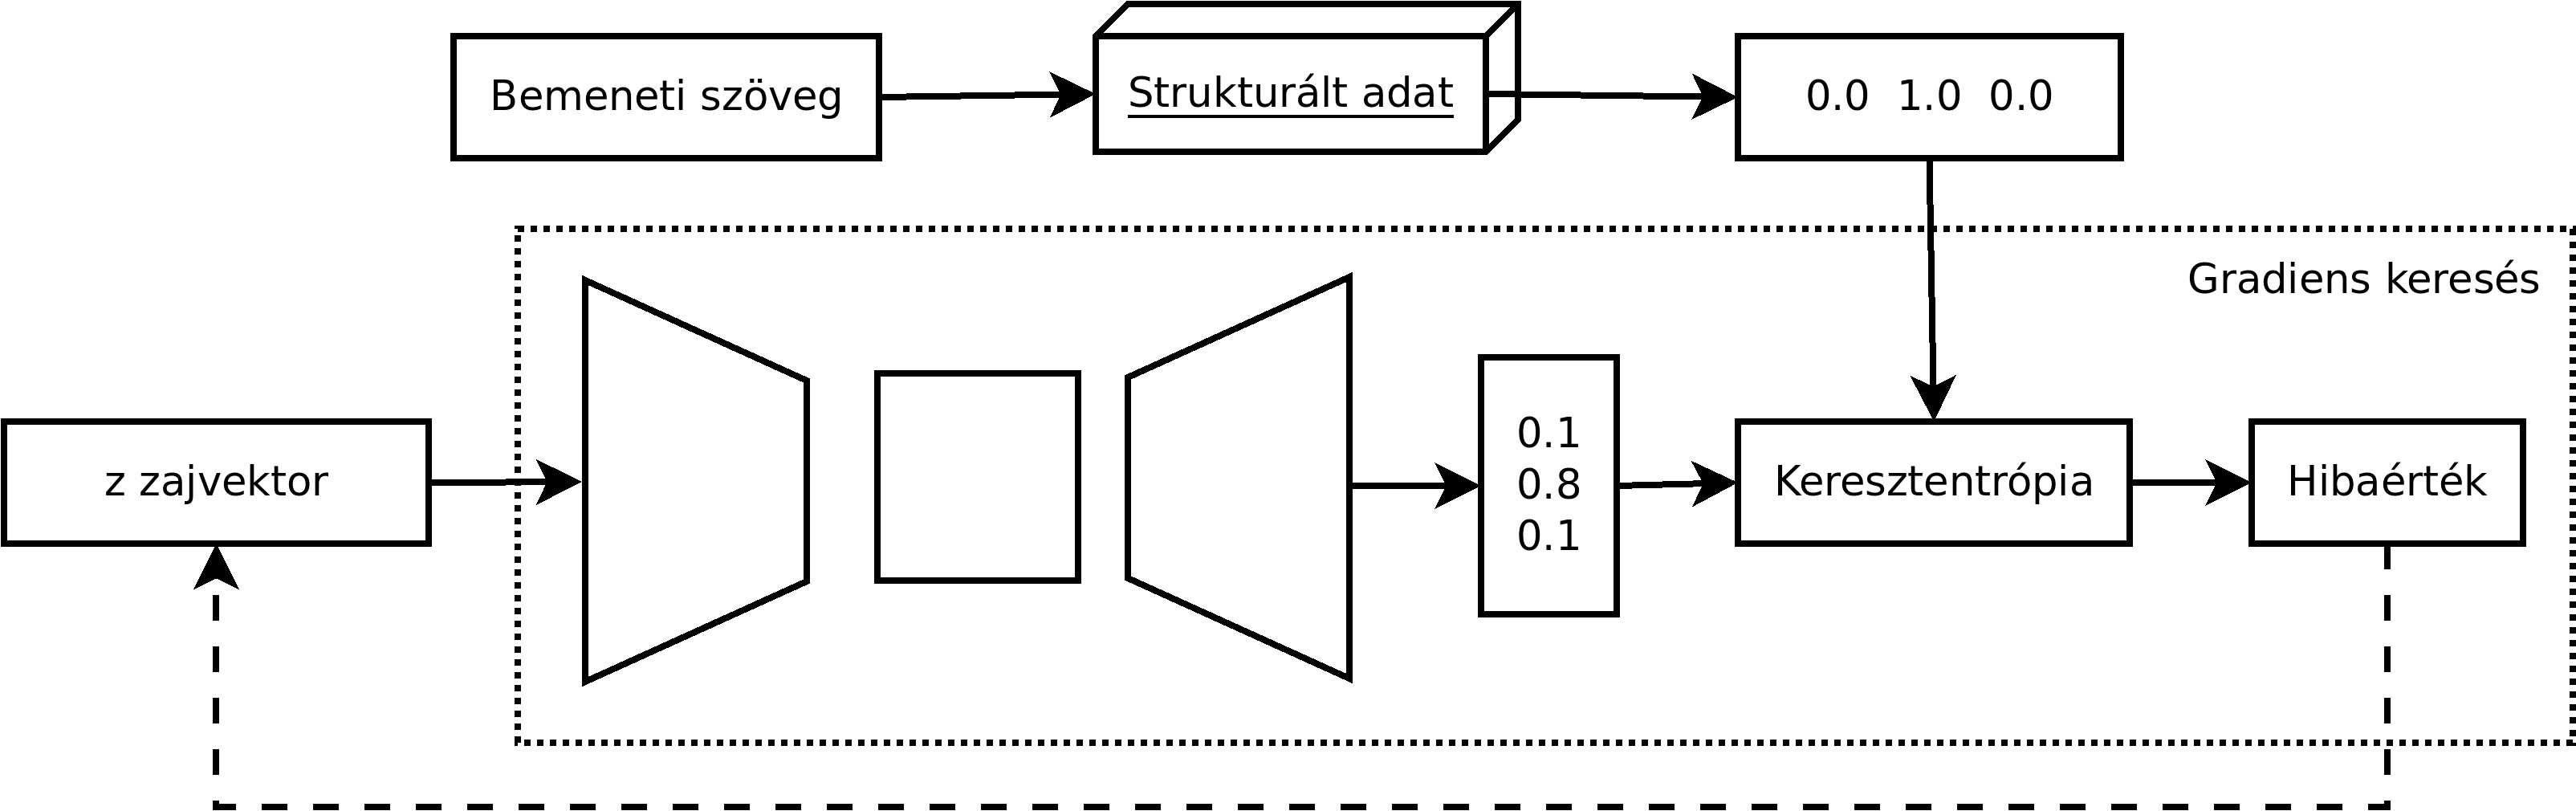
\includegraphics[width=15cm]{images/architecture.png}
\caption{Architektúra}
\label{fig:architecture}
\end{figure}



% \Section{A fejezet célja}
% Ez a fejezet még nem a saját eredményekkel foglalkozik, hanem bemutatja, mi a problémakör, milyen módszerekkel, milyen eredményeket sikerült elérni eddig másoknak.
% TODO: Problémakör bemutatása, különböző szerzők eredményeinek ismertetése
% A hivatkozások jelentős része ehhez a fejezethez szokott kötődni.
% (Egy hivatkozás például így néz ki \cite{coombs1987markup}.)
% Ez szintén egy példa internetes hivatkozásra, a CSS szabvány kapcsán \cite{css}.
% Itt lehet bemutatni a hasonló alkalmazásokat.

% \Section{Tartalom és felépítés}
% A fejezet tartalma témától függően változhat. Az alábbiakat attól függően különböző arányban tartalmazhatják.
% \begin{itemize}
% \item Irodalomkutatás. Amennyiben a dolgozat egy módszer kidolgozására, kifejlesztésére irányul, akkor itt lehet részletesen végignézni (módszertani vagy időrendi bontásban), hogy az eddigiekben milyen eredmények születtek a témakörben.
% \item Technológia. Mivel jellemzően kutatásról vagy szoftverfejlesztésről van szó, ezért annak a jellemző elemeit, technikai részleteit itt kell bemutatni.
% Ez tehát egy módszeres bevezetés ahhoz, hogy ha valaki nem jártas a témakörben, akkor tudja, hogy a dolgozat milyen aktuálisan elérhető eredményeket, eszközöket használt fel.
% \item Piackutatás. Bizonyos témáknál új termék vagy szolgáltatás kifejlesztése a cél.
% Ekkor érdemes annak alaposan utánanézni, hogy aktuálisan milyen eszközök érhetők el a piacon.
% Ez szoftverek esetében a hasonló alkalmazások bemutatását, táblázatos formában történő összehasonlítását jelentheti.
% Szerepelhetnek képek és észrevételek a viszonyításként bemutatott alkalmazásokhoz.
% \item Követelmény specifikáció. Külön szakaszban érdemes részletesen kitérni az elkészítendő alkalmazással kapcsolatos követelményekre.
% Ehhez tartozhatnak forgatókönyvek (\textit{scenario}-k).
% A szemléletesség kedvéért lehet hozzájuk képernyőkép vázlatokat is készíteni, vagy a használati eseteket más módon szemléltetni.
% \end{itemize}

% \Section{Amit csak említés szintjén érdemes szerepeltetni}
% Az olvasóról annyit feltételezhetünk, hogy programozásban valamilyen szinten járatos, és a matematikai alapfogalmakkal sem ebben a dolgozatban kell megismertetni.
% A speciális eszközök, programozási nyelvek, matematikai módszerekk és jelölések persze jó, hogy ha említésre kerülnek, de nem kell nagyon belemenni a közismertnek tekinthető dolgokba.



\Section{Tensorflow és Keras}

A dolgozat programjának megvalósításához a TensorFlow függvénykönyvtárat választottam ki. A TensorFlow egy ingyenes, open-source gépi tanulásra használatos függvénykönyvtár, amely elsősorban mély- és gépi-tanulásos alkalmazások implementálására használatos. Számos programozási nyelvhez érhető el az API-ja, beleértve a Python, Java, C++ és JavaScript nyelveket. Viszont az API fő fejlesztési iránya a Python nyelvre öszpontosul. A könyvtár a Google Brain fejlesztésében született meg 2015-ben, majd 2019-ben megjelent a 2.0-ás API verzió is, amely az API váltásból adódóan visszafelé nem teljesen kompatibilis az elsővel. Jelenleg a 2.8-as számozású stabil kiadással rendelkezik, a dokumentációja a \cite{tensorflow} forrás alatt érhető el. Az API lehetőséget ad az elosztott tanításra is. A betanított modellek széleskörben alkalmazhatóak, akár web- vagy mobilalkalmazásokba is integrálhatóak. 

A Keras függvénykönyvtár egy interfészt biztosít a TensorFlowhoz. Segítségével igazán egyszerűen, modulárisan és átláthatóan állíthatunk össze neurális hálózatokat. Az általa biztosított eszközkészlet igazán változatos. A modellek összeállítására is többféle lehetőségünk van, például a \textit{Sequential API} használatával pipeline szerű modelleket építhatünk a különféle rétegek egymás után illesztésével. A \textit{Functional API} segítségével pedig igazán komplex kapcsolatokkal rendelkező architektúrák is megvalósíthatóak, a kódbonyolultság növekedése nélkül. A Keras korábban több backendet is támogatott, viszont a legrissebb verzióiban csak a TensorFlow-hoz alkalmazható. Látható, hogy a két könyvtár mennyire összefonódott. A dokumentációja a \cite{keras} forrás alatt érhető el.

TODO: Keras és Tenforflow 2 bemutatása, példákkal, ábrákkal

Python-hoz a \texttt{tensorflow} csomag az alábbi kódrészlettel importálható. A TensorFlow tartalmazza a Keras-t modul formájában. Amennyiben nem importáljuk be külön a modult, úgy a \texttt{tf.keras}-al is elérhetjük, viszont az alábbi kódrészletben a Keras is importálásra kerül. A dolgozatban található kódrészleteknél az alábbi két sort nem tűntetem fel a továbbiakban, egységesen minden kódrészlethez az alábbiak szükségesek, a kivételt képző eseteknél, ahol szükséges lehet további csomagok importálása is, külön ki fogom emelni. (nem biztos, hogy lesz ilyen...)
\begin{python}
import tensorflow as tf
from tensorflow import keras
\end{python}

\Section{Modellek tanítása}

A mély neurális hálózatok tanítása igazán erőforrásigényes feladat. A tanítható paraméterek nem ritkán milliós nagyságrendűek, a dataset-eknek pedig kellően nagynak kell lenniük, a feldolgozandó adatoknak a memóriába is bele kell férnie. Egy-egy iteráció igen sok időbe tellhet egy gyengébb hardveren.

Az első demóprogramok futtatása során szembesültem az első nehézséggel: A laptopom nem a legalkalmasabb a modellek tanítására, hiszen igen sok időt vett igénybe a legkisebb példák futtatása is. Az interneten felleltem a Google Colab környezetet, amely ingyenes virtuális környezetet biztosít a python notebook-ok szerkesztéséhez és futtatásához, egy előre meghatározotlan ideig GPU-t (Tesla K80) és TPU-t is biztosít. Az ingyenes verzióban a napi GPU használatának limitje nincsen meghatározva, így egy idő után lekapcsolhatják és GPU nélkül megnövekszik a tanítás hossza. Az ingyenes verzióban a környezetet 12 óránként resetelik, így minden adat elvezhet, továbbá csak akkor futhat a script, ha meg van nyitva a böngészőablak. Természetesen a Tensorflow és a Keras ajánl lehetőségeket a modellek mentésére vagy a tanítás közbeni checkpoint-ok készítésére.

Például az alábbi kód segítségével tetszőleges attribútumokkal létrehozhatunk egy checkpoint objektumot, amely segítségével mentéseket csinálhatunk a checkpointben meghatározott objektumok állapotairól. Amelyeket a tanítás folytatásához később be is tölthetünk.
\begin{python}
checkpoint = tf.train.Checkpoint(
    generator_optimizer=generator_optimizer,
    discriminator_optimizer=discriminator_optimizer,
    generator=generator,
    discriminator=discriminator
)
\end{python}

Egy másik lehetőségként lementhetjük a teljes modellt, amelyet később egyszerűen be is tölthetünk.
\begin{python}
model.save("./my_model")

new_model = keras.models.load_model("./my_model")
\end{python}
Viszont számomra a Google Colab ingyenes próbaverziója nem volt teljesen megfelelő, a kiszámíthatatlanság miatt. Magyaroroszágon jelenleg nem is lehet előfizetni, így újabb felületet kellett keresnem. Egy fórumon böngészve találtam rá a Kaggle felületre, amely hasonló környezetet kínál, mint a Colab. Viszont az általa biztosított virtuális környezet hardvere jobbnak bizonyult a Colab-ben használhatóaknál. A GPU használat heti szinten kerül meghatározásra órákban, ami csak a használat során számolódik. Továbbá lehetőséget kínál a notebookok ütemezett futtatására is és az Kaggle-ön megtalálható bármelyik datasetet könnyedén betölthetjük és használhatjuk. Mindezen előnyök miatt a Kaggle-t választottam a modelljeim tanítására.

Az alábbi táblázatban található meg a laptopom és a Kaggle által biztosított környezet specifikációi:
\begin{center}
\begin{tabular}{ p{1.2cm}||p{6cm}|p{6cm}  }
	  & Dell Insprion-5558 & Kaggle környezet\\
	\hline
	\textbf{CPU} & 4x Intel(R) Core(TM) i3-5005U CPU @ 2.00GHz & 2x Intel(R) Xeon(R) CPU @ 2.00GHz\\
	\textbf{RAM} & 2x 4GB DDR3 1600 MHz & 15GB\\
	\textbf{GPU} & Intel HD Graphics 5500 (VGA) & Nvidia Tesla P100-PCIE-16GB\\
	\textbf{HDD} & 1TB & 73GB
\end{tabular}
\end{center}
A három környezet (laptop, Colab, Kaggle) teljesítményét egy általam felállított méréssel vizsgáltam.
A \texttt{RuntimeMeasure.ipynb} notebook használatos a teljesítménymérés elvégzéséhez.
A teljesítménymérés alapja egy olyan GAN hálózat, amelyet meghatározott paraméterekkel hozunk létre.
A tanítás során az alábbi paraméterek változatlanok:
\begin{center}
\begin{tabular}{ c|c|c|c }
	Látens dimenziószám & mini-batch méret & filterek száma & kernelméret\\
	\hline
	100 & 32 & 128 & ($3\times 3$)
\end{tabular}
\end{center}
A felbontásnövelő rétegek száma a futó paraméter, amelyet 0-tól 3-ig vizsgálunk.
A hálózat felépítése megegyezik a DCGAN architektúrával, azzal az eltéréssel, hogy a Generátor utolsó dekonvolúciós rétege helyett egy konvolúciós réteg található, amely csupán dimenziócsökkentési feladatot végez, vagyis a feature-öket a három színcsatornába transzformálja. Hasonlóan a Diszkriminátorban is, az első konvolúciós réteg a bemeneti kép csatornáit bővíti ki, nem végez kicsinyítést.
A hálózatot 5 epoch-ig tanítjuk az adott felbontásnövelő rétegek mellett, majd az átlagos futásidő kerül lejegyzésre.
A mérés során a hálózatot a Cifar10 \cite{krizhevsky2009learning} adathalmazon tanítottam, labelek nélkül a train részhalmazán, amely 50000 képet tartalmaz. Az adathalmaz képei ($32 \times 32$) felbontásúak és 3 színcsatornával rendelkeznek (rgb). Összesen 10 féle osztályba sorolhatjuk be az adathalmaz elemeit.
A mérés egyes állomásain a generátor különféle felbontásokban generálja a képeket. Így a tanítás előtt a tanítóhalmaz képeit is a generátor kimenetével megegyező méretekre kell skáláznunk.

A generátor kimenete a felbontásnövelő rétegek számával változik. Ha nem alkalmazunk ilyen réteget, akkor az ($4 \times 4$) felbontású képeket eredményez, majd rendre 1 réteg esetén ($8 \times 8$), 2 réteg esetén ($16 \times 16$) és 3 réteg esetén ($32 \times 32$) felbontású képek jelennek meg a generátor kimenetén. A diszkriminátort is ennek megfelelően át kell alakítanunk, ott viszont a felbontáscsökkentő rétegek számát kell módosítanunk. Mivel a felvázolt GAN szimmetrikus, így a felbontásnövelő és felbontáscsökkentő rétegek száma megegyezik.

\begin{python}
...
for i in range(upsampling_layers):
    hidden = keras.layers.Conv2DTranspose(
        units_per_layer, kernel_size, 2, 'same'
    )(hidden)
    hidden = keras.layers.BatchNormalization()(hidden)
    hidden = keras.layers.ReLU()(hidden)
...
\end{python}

A generátorban és a diszkriminátorban is egy-egy for ciklussal megoldhatjuk az említett rétegek hozzáadását a hálók építése során. A fenti példa kód szemlélteti a generátorban lévő dekonvolúciós réteg hozzáadását.
A notebookot futtatva a \ref{fig:runtime} ábrán látható eredmények jöttek ki.

\begin{figure}[h]
\centering
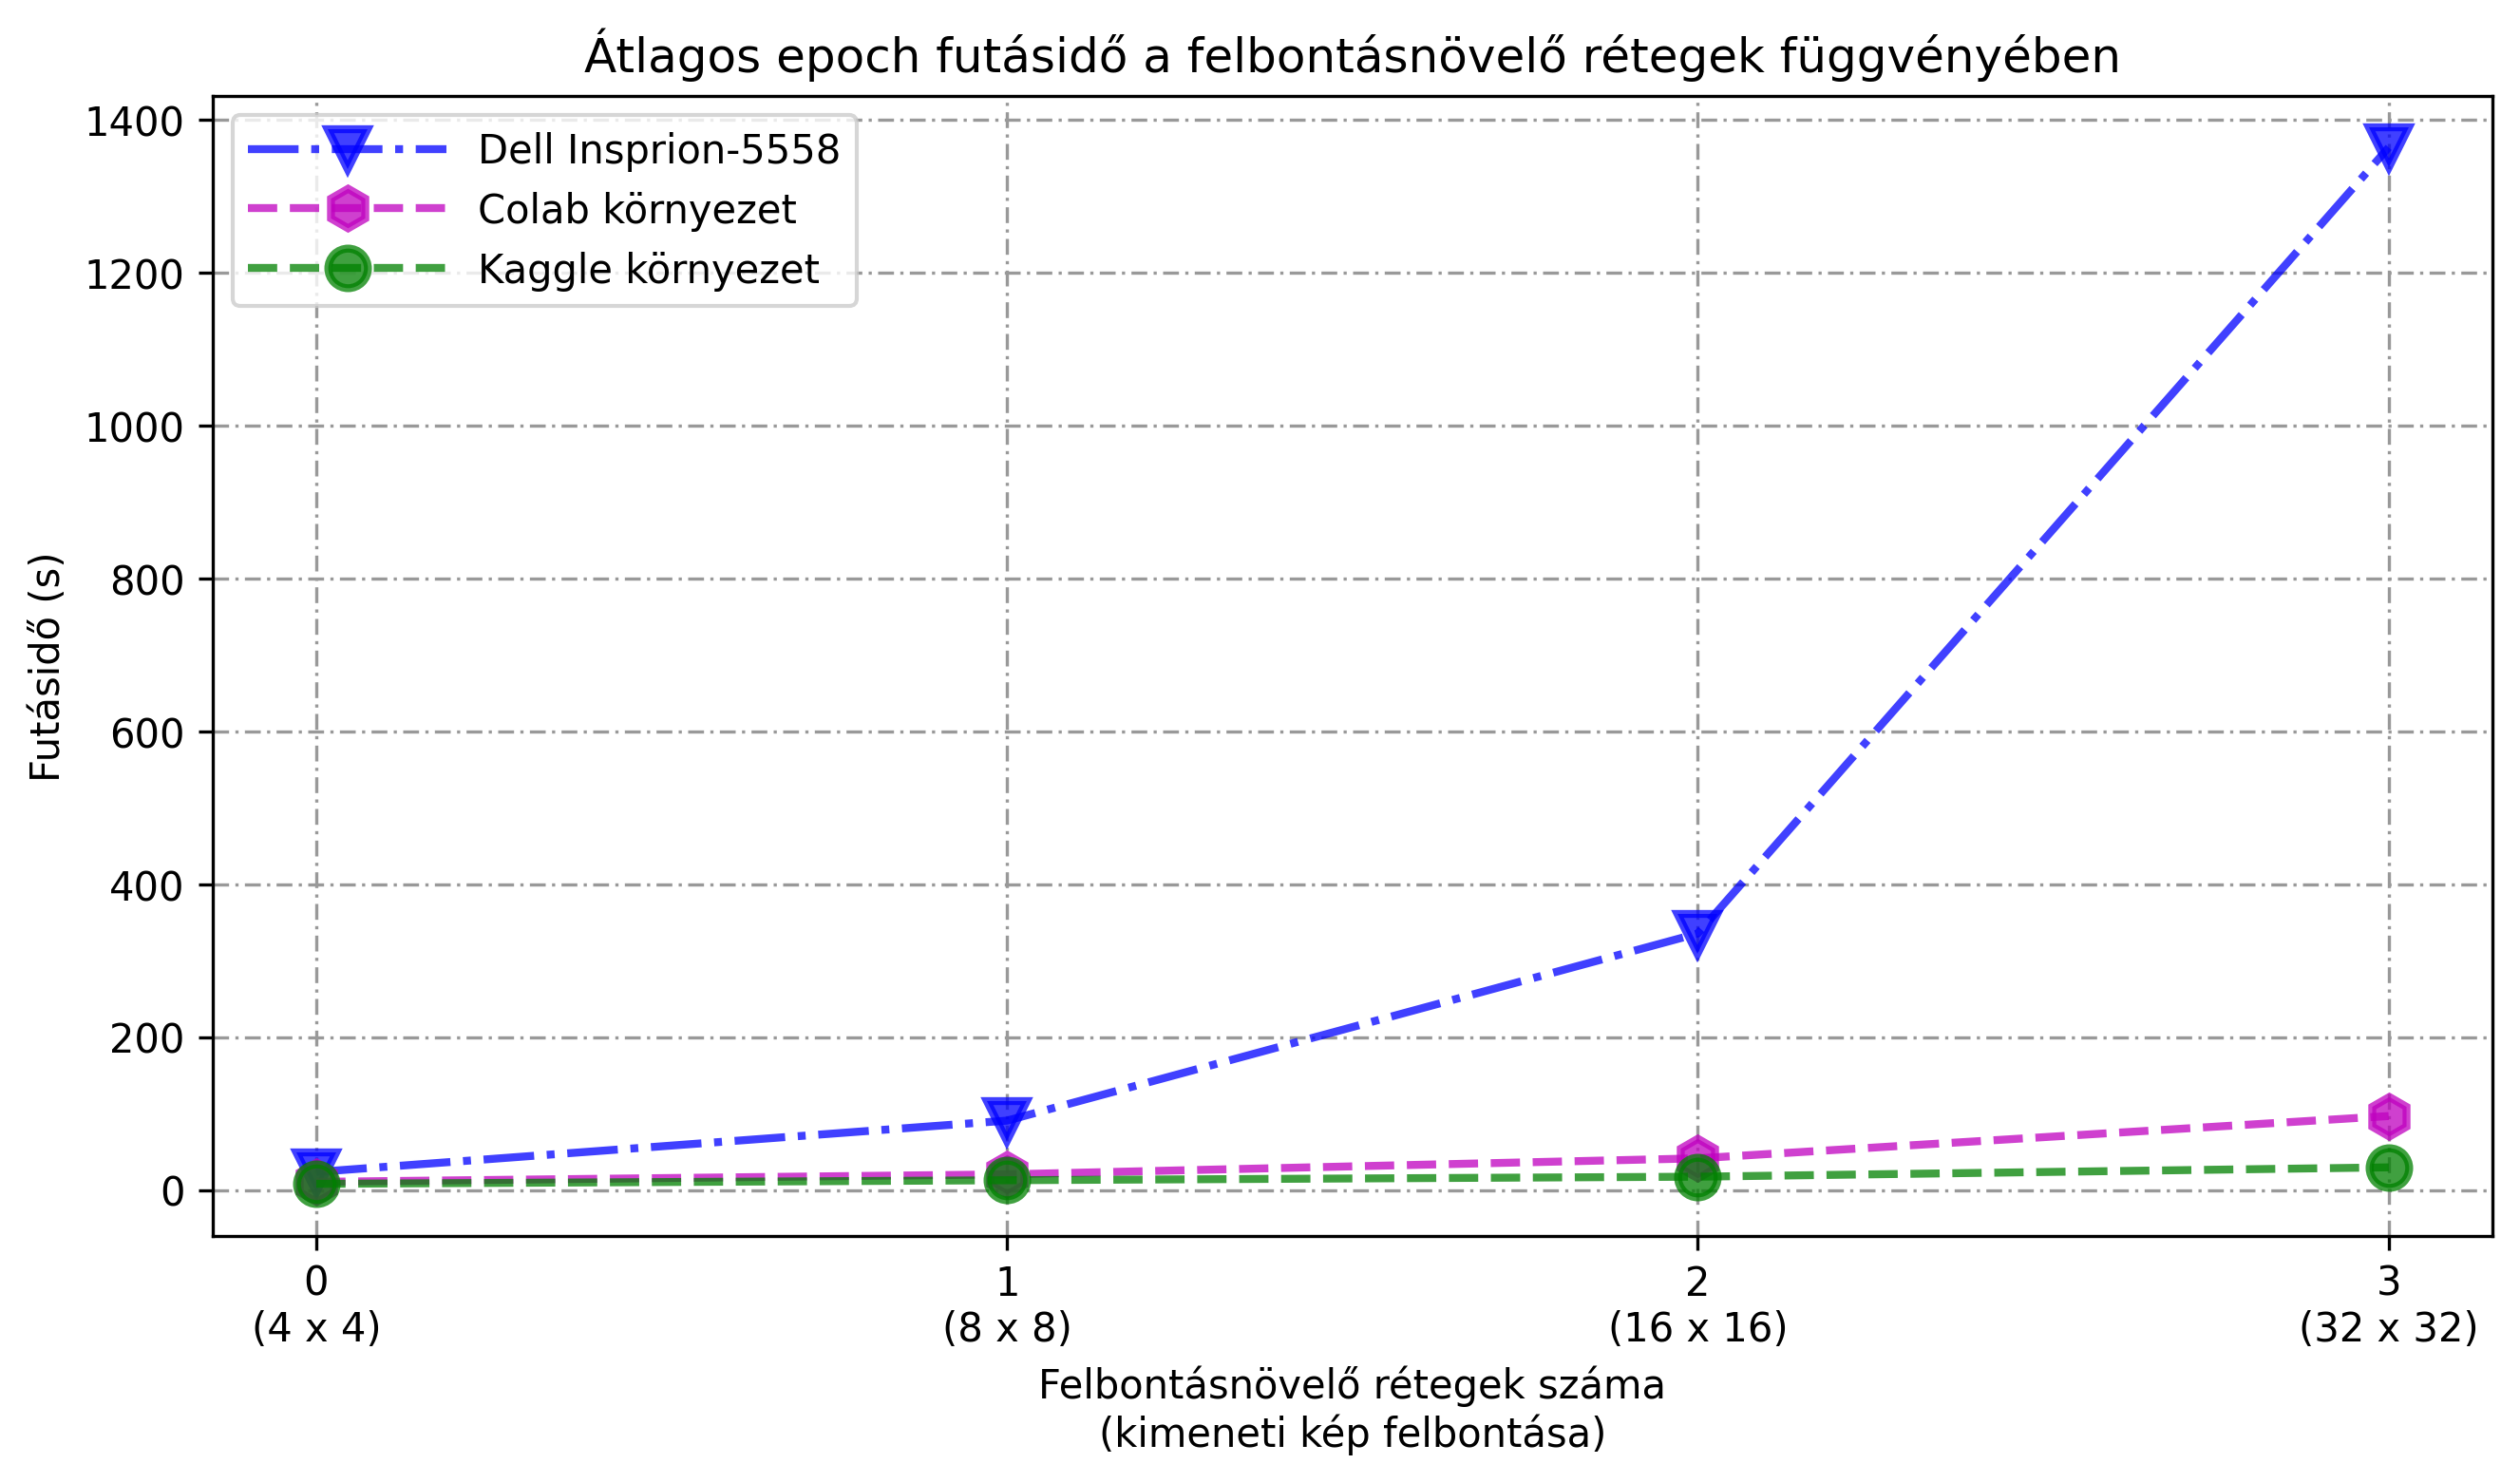
\includegraphics[width=15cm]{images/runtime.png}
\caption{Runtime ábra}
\label{fig:runtime}
\end{figure}

Mint látható, a laptopom igen alulmaradt a két virtuális környezettel szemben.


A dolgozat terjedelme (a mellékletek nélkül számítva) diplomamunka esetén 60-90, szakdolgozat esetén 40-60 oldal között optimális.

Az alábbi tagolás sorrendjének betartása nem kötelező, de az arányok lényegesek!
\begin{enumerate}
	\item Bevezető\\
Feladat ismertetése, honnan jött az ötlet, kitőzött célok, követelmények, elvárások. (~ 2 oldal)
	\item Irodalom feldolgozás, háttér információk (~ 10\%, de elméleti területen írt dolgozatok esetében ez akár 30\% is lehet)
	\begin{itemize}
		\item Ha cég megbízásából dolgozunk, ebben a részben lehet ismertetni a vállalatot. 
		\item Elméleti háttér ismertetése, hivatkozva a felhasznált irodalomra. 
	\end{itemize}
	\item A feladat megoldásához rendelkezésre álló technikák, technológiák, fejlesztőeszközök ismertetése, összehasonlítása, (előnyök, hátrányok ütköztetése, felhasználhatóság mérlegelése). (~ 25\%)
	\item Saját teljesítmény előállításához ténylegesen felhasznált eszközök részletes ismertetése; a kiválasztás szempontjai, telepítés, használatba vétel előfeltételei és lépései (ha azok nem magától értetődők). (~ 20\%)
	\item Saját munkánk (alkalmazásfejlesztés, mérés, tervezés stb.) részletes leírása, az eredmények szemléletes ismertetése. (~ 35\%)
	\item Összegzés\\ Tapasztalatok, eredmények összegzése; a feladat elkészítése során felmerült nehézségek, elkövetett hibák; jövőbeni fejlesztési lehetőségek. (~10\%)
\end{enumerate}